\section{Results}
\label{sec:results}

\subsection{CPU implementation check}

The current local run is reported only as a software-verification milestone.
Across three source scenes and 35 fault variants per scene, the benchmark
created 105 cases containing 141 expected rule findings. The validator recovered
all expected findings without an additional finding under the registered
ground truth. The fixed whitelisted-tool implementation returned 102 cases to a
valid state and escalated the three unsupported-friction cases. Validation and
repair were sub-millisecond in this small CPU check, but those timings vary
with host load and are retained in the run report rather than treated as a
performance result.

The same implementation check compared the task-activated root with an
all-loaded root over three-zone fixtures. Task activation reduced composed
prim count by 20--25\%, rigid-body and collider count by 40--50\%, and bytes in
used USD layers by 18.0--24.5\%. These are structural consequences of the
fixture and confirm that the two composition conditions differ as intended;
they are not substitutes for RTX load-time, memory, and collision-query
measurements.

These values should not be interpreted as evidence that the method generalizes
to unseen construction scenes. The fault operators were written against the
same explicit contract as the validator, and the fixed repair implementation
had access to trusted source evidence. Their purpose is to verify rule
coverage, compound-fault accounting, audit generation, and the distinction
between safe repair and escalation before the held-out and language-model
comparisons are executed.

\subsection{Humanoid task outcomes under scene-model feature defects}
\label{sec:task-outcomes}

\begin{figure*}[t]
\centering
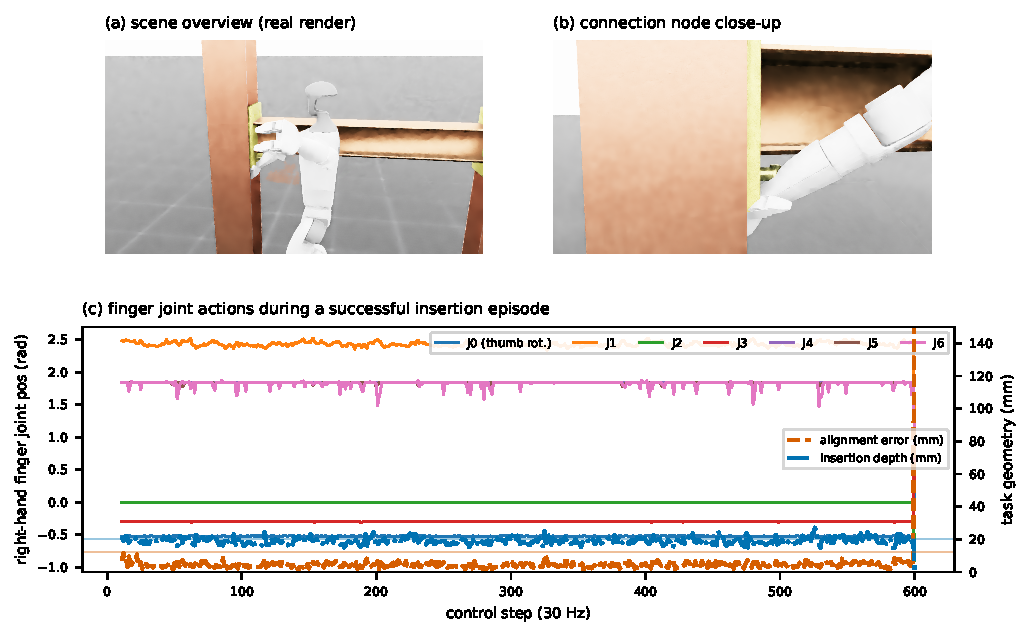
\includegraphics[width=\textwidth]{figures/fig10_experimental_setup.pdf}
\caption{Experimental setup and executor action stream. (a)--(b) True
simulator renders of the two-column portal-frame assembly scene: the overview
shows the G1 working at the end plate of the supported beam; the close-up
shows the $2\times2$ bolt group on the collision-enabled plate. (c) Right-hand
finger joint positions and task geometry over one successful insertion
episode: the policy closes the fingers early and holds a power grasp while the
transport--align--insert phases proceed; the alignment error (dashed) and
insertion depth (dash-dot) reference lines use the right axis. Frames and
trajectories are generated by the registered capture scripts.}
\label{fig:experimental-setup}
\end{figure*}

The runtime executor for the defect-consequence study is a frozen
reinforcement-learning insertion policy on the \texttt{Isaac-Assembly-G1-v2}
task: a Unitree G1 with a locked lower body transports a virtual-grasped M20
bolt and inserts it along the horizontal axis into the lower-right hole of a
$2\times2$ bolt group on the beam end plate of a two-column portal frame
(\Cref{fig:experimental-setup}). The plate carries collision geometry with the
four holes cut out, so both the hand and the bolt are physically blocked
outside the holes; the bolt may pass only through the hole circle. Success
follows the same criterion as the training reward: transverse alignment error
below 12\,mm and insertion depth of at least 20\,mm from the plate surface.
The checkpoint used (fine-tuned on this scene) achieves 85.5\% success over
200 evaluation episodes (87.0\% over 1000) without injected defects.
\Cref{fig:task-sequence} shows one successful execution sequence of this
executor in the defect-free scene.

\begin{figure*}[t]
\centering
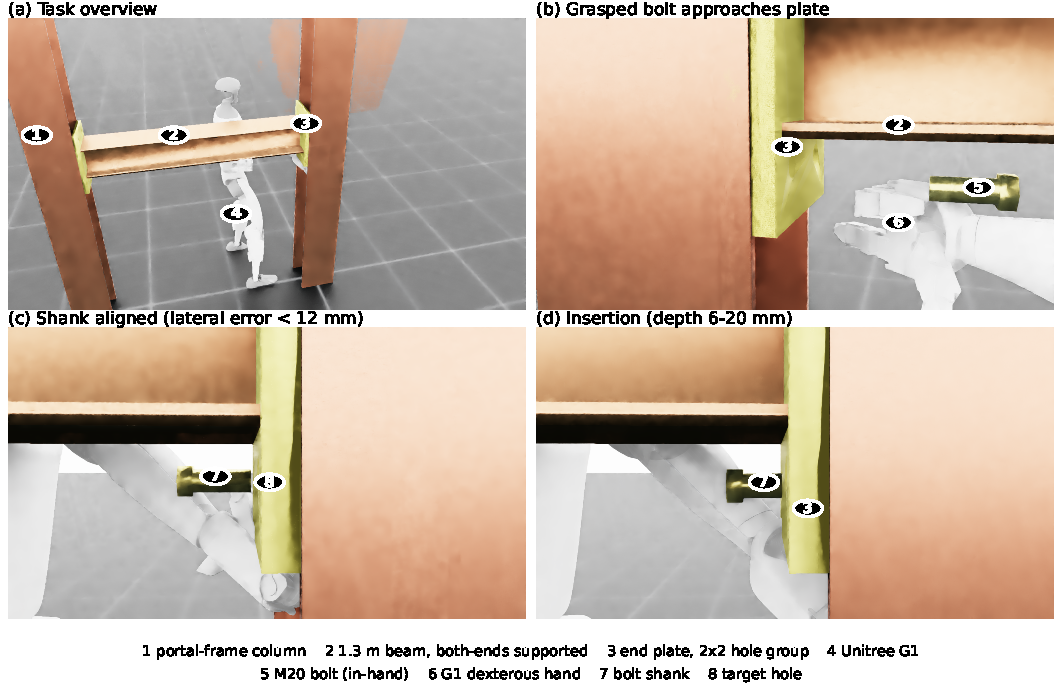
\includegraphics[width=\textwidth]{figures/fig11_task_sequence.pdf}
\caption{Executed insertion sequence of the frozen policy in the defect-free
scene (true simulator renders, captured at 2560$\times$1440). (a) Task
overview: the G1 stands at the end plate of the 1.3\,m beam, which is
supported at both ends by the two-column portal frame. (b) The right hand
transports the virtually grasped M20 bolt toward the plate. (c) The shank is
aligned with the lower-right hole of the $2\times2$ group (transverse error
below 12\,mm). (d) Insertion proceeds along the hole axis; success requires
a depth of at least 20\,mm from the plate surface. Numbered markers identify
the scene features listed in the legend at the bottom of the figure. All
frames are captured from one successful evaluation episode by the registered
panel-capture script.}
\label{fig:task-sequence}
\end{figure*}

Defects from the six feature families of \Cref{sec:experiments} were injected
at episode reset as controlled deviations between the scene model observed by
the policy and the ground-truth insertion target, at graded severities. All
conditions share one frozen policy, one seed partition, and an identical
episode-randomization stream: the injection events consume the same amount of
randomness whether or not a defect is active, so episode $k$ under any defect
condition is the exact paired replicate of episode $k$ under the defect-free
baseline. Paired binary outcomes are compared with exact two-sided McNemar
tests; $b$/$c$ denote episodes that changed from success to failure and from
failure to success, respectively. Two defect classes are distinguished
throughout: \emph{information defects} leave the physical scene intact but
corrupt what the controller can know or assume (geometry, semantic identity,
task reference, construction state), whereas the \emph{interface-clearance}
conditions change the physically executable task itself (an emulation of
jamming, not a contact-mechanics simulation). In total 10{,}600 paired
episodes were run (14 conditions $\times$ 2 seed partitions $\times$ 200
episodes, plus five geometry conditions at 1000 episodes for power); every
figure and table
is generated from the per-episode ledgers by the registered scripts.

\begin{table*}[t]
\centering
\caption{Insertion outcome under injected scene-model feature defects (200
paired episodes per condition, seed 42; geometric conditions repeated with
1000 paired episodes). \emph{Reward success} is the training-reward criterion
(transverse error below 12\,mm, depth at least 20\,mm). \emph{Geometric
valid} is the stricter criterion recomputed per episode from the ledger
(transverse error within the 1\,mm nominal radial clearance \emph{and} depth
at least 20\,mm): whether the bolt actually passed the hole, not merely
satisfied the reward. $\Delta$pp is the reward-success change relative to the
defect-free baseline of the same batch. Significance: exact McNemar test on
reward success, ${***}\,p<0.001$, ${**}\,p<0.01$, ${*}\,p<0.05$.}
\label{tab:defect-decay}
\small
\resizebox{\textwidth}{!}{%
\begin{tabular}{p{0.17\textwidth}p{0.22\textwidth}cccccc}
\toprule
Feature family & Injected defect & Reward success & Geometric valid &
$\Delta$pp & $b$/$c$ & $p$ \\
\midrule
-- & none (baseline) & 85.5\% & 75.5\% & -- & -- & -- \\
Geometry, hole position & $\pm$2\,mm, random direction & 85.0\% & 63.0\% & $-$0.5 & 3/2 & n.s. \\
Geometry, hole position & $\pm$5\,mm & 86.5\% & 46.5\% & $+$1.0 & 2/4 & n.s. \\
Geometry, hole position & $\pm$10\,mm & 76.0\% & 14.0\% & $-$9.5 & 21/2 & *** \\
Geometry, member pose & whole node $+$10\,mm & 82.0\% & 72.5\% & $-$3.5 & 10/3 & n.s. \\
Assembly interface & radial clearance 0.75\,mm & 33.5\% & 33.5\% & $-$52.0 & 104/0 & *** \\
Assembly interface & radial clearance 0.5\,mm & 21.5\% & 22.0\% & $-$64.0 & 128/0 & *** \\
Assembly interface & radial clearance 0.25\,mm & 5.5\% & 5.5\% & $-$80.0 & 160/0 & *** \\
Semantic identity & label missing (nominal prior only) & 13.0\% & 1.0\% & $-$72.5 & 145/0 & *** \\
Semantic identity & label wrong (plate centre, no hole) & 0.0\% & 0.0\% & $-$85.5 & 171/0 & *** \\
Task reference & wrong hole of the $2\times2$ group & 0.0\% & 0.0\% & $-$85.5 & 171/0 & *** \\
Construction state & member not yet in place & 0.0\% & 0.0\% & $-$85.5 & 171/0 & *** \\
Physical properties & bolt mass $\times0.5$ / $\times2$ & 85.5\% & 75.5\% & $+0.0$ & 0/0 & n.s. \\
\bottomrule
\end{tabular}
}
\end{table*}

\Cref{tab:defect-decay} yields a clear criticality ordering. Symbolic and
referential features---task references, construction states, and semantic
identity---are discretely fatal: a single wrong reference drives success to
zero because the executor's target is defined by them. Among continuous
features, the assembly interface dominates: shrinking the effective radial
clearance of the nominal \O22\,mm hole from 1\,mm to 0.75\,mm halves-plus
success (85.5\% $\rightarrow$ 33.5\%), and 0.25\,mm is nearly fatal.

The geometric family separates two effects that are easily conflated, and the
answer depends on executor precision. A 10\,mm error in the \emph{absolute}
pose of the whole connection node is partly compensated by the policy's
closed-loop perception ($-$3.5\,pp, $b$/$c$=10/3, n.s.\ at $n$=200), while the
same 10\,mm applied to the hole position \emph{relative to the observed
member}---the quantity the scene model certifies and the policy cannot
see---costs $-$9.5\,pp ($p<0.001$). At 1000 paired episodes both effects are
significant but remain separable in magnitude (member $-$7.0\,pp, hole
$-$7.9\,pp against the 87.0\% baseline), while 2 and 5\,mm hole errors stay
inside the executor's tolerance band (86.4\% and 86.6\%, n.s.).

\paragraph{Reward success versus geometric validity.}
The 12\,mm reward threshold is an information-chain criterion, not a
certificate of physical insertability: the nominal \O22\,mm hole leaves only
1\,mm radial clearance for the M20 bolt. Recomputing each episode under a
strict geometric criterion (transverse error within the 1\,mm clearance
\emph{and} depth at least 20\,mm) separates the two and, where they diverge,
sharpens rather than softens the ordering above. The defect-free executor
reaches 75.5\% geometric-valid against 85.5\% reward success---about ten
points of reward successes are motion completions that never achieve the
geometric bound. Anchor-relative hole errors, which the reward criterion
partly absorbs, become strongly consequential geometrically: geometric-valid
falls to 63.0\% at 2\,mm, 46.5\% at 5\,mm and 14.0\% at 10\,mm, so the
certified hole coordinate is the dominant geometric quantity once physical
insertability is required. In contrast, absolute member-pose error stays
largely correctable (72.5\% geometric-valid at 10\,mm). A paired McNemar test
between the two 10\,mm conditions under the geometric criterion confirms the
separation is decisive, not marginal ($b$=570 versus $c$=47,
$p=3.6\times10^{-115}$). The interface-clearance conditions are unchanged
between the two criteria, because their explicit geometric gate already
enforces the physical bound. The loose reward threshold therefore masks
geometric failure precisely for the information family the scene model is
responsible for certifying, which is the empirical reason interface
coordinates require certified values with provenance
(\Cref{sec:discussion}).

Physical-property defects (bolt mass $\times0.5$ and $\times2$) produced
bit-identical outcomes ($b$/$c$=0/0). This null result is structural, not
statistical: the executor's virtual-grasp scaffold makes the bolt kinematic,
so mass and friction have no dynamical channel in this task stage. We
therefore report the physical family as \emph{not consequential for the
transport-and-insert motion chain} and defer its force-level criticality to a
full-contact ablation (\Cref{sec:discussion}).

All findings replicate under a second seed partition (seed 123, 200 paired
episodes per condition): success rates deviate by at most 3.5\,pp from the
seed-42 values and effect directions match in every condition, with one
exception worth noting---the borderline 10\,mm member-pose effect is
significant in the powered run but not at $n$=200 under either seed,
illustrating why we report effect sizes with confidence statements rather than
significance alone (\Cref{sec:discussion}).


\placeholder{Do not write narrative results before the registered scripts have
generated the final tables. Populate this section in the following order:
(1) compiler fidelity, (2) validator detection, (3) repair outcomes,
(4) multi-scale efficiency, (5) humanoid task outcomes --- now reported in
\Cref{sec:task-outcomes}, (6) ablations, and (7) failure cases.}

\begin{figure*}[t]
\centering
\plannedfigure{42mm}{Figure 7 production placeholder: detection and repair results}{
Panel (a): paired point or forest plot of critical-fault recall and F1 by
method and fault family with bootstrap 95\% confidence intervals. Panel (b):
valid repair, incorrect repair, and escalation proportions. Panel (c):
distribution of repair iterations and wall-clock time. Use identical method
ordering and a colour-blind-safe palette, with symbols or line styles in
addition to colour.}{
\texttt{detection\_repair.csv} generated by the registered experiment script.
Python plotting source; editable SVG and embedded-font PDF.}
\caption{Detection and repair performance across scene-fault families and
comparison methods. Confidence intervals and paired comparisons will be
computed over the frozen benchmark partition.}
\label{fig:detection-repair-results}
\end{figure*}

\begin{table*}[t]
\centering
\caption{Primary detection and repair outcomes. Values will be imported from
the registered result file; no manuscript cell will be edited manually.}
\label{tab:detection-repair}
\small
\resizebox{\textwidth}{!}{%
\begin{tabular}{p{0.19\textwidth}ccccccc}
\toprule
Method & Precision & Recall & Critical recall & Valid repair & Incorrect
repair & Escalation & Time \\
\midrule
Direct conversion & \placeholder{TBD} & \placeholder{TBD} &
\placeholder{TBD} & n/a & n/a & n/a & \placeholder{TBD} \\
Fixed-rule conversion & \placeholder{TBD} & \placeholder{TBD} &
\placeholder{TBD} & \placeholder{TBD} & \placeholder{TBD} &
\placeholder{TBD} & \placeholder{TBD} \\
Free-form agent & \placeholder{TBD} & \placeholder{TBD} &
\placeholder{TBD} & \placeholder{TBD} & \placeholder{TBD} &
\placeholder{TBD} & \placeholder{TBD} \\
Full method & \placeholder{TBD} & \placeholder{TBD} &
\placeholder{TBD} & \placeholder{TBD} & \placeholder{TBD} &
\placeholder{TBD} & \placeholder{TBD} \\
\bottomrule
\end{tabular}
}
\end{table*}

\begin{figure*}[t]
\centering
\plannedfigure{42mm}{Figure 8 production placeholder: efficiency and task consequence}{
Panel (a): paired active prim count, peak memory, and scene-load time for
all-loaded and task-activated composition. Panel (b): readiness score versus
humanoid task success with a logistic fit and 95\% confidence band. Panel (c):
failure-cause composition, separating scene-model, planning, control, and
contact failures. Use dots and intervals rather than decorative bars.}{
\texttt{resource\_efficiency.csv} and \texttt{task\_outcomes.csv} from RTX
batch runs. Python source, SVG/PDF, and a data-to-mark audit test.}
\caption{Resource effect of task-activated composition and the relationship
between scene readiness and downstream humanoid assembly outcomes.}
\label{fig:efficiency-task-link}
\end{figure*}

\begin{table*}[t]
\centering
\caption{Runtime resource use and task-level outcomes. The final table will
report estimates with 95\% confidence intervals and explicit denominators.}
\label{tab:runtime-task}
\small
\resizebox{\textwidth}{!}{%
\begin{tabular}{p{0.17\textwidth}cccccccc}
\toprule
Condition & Active prims & Peak memory & Load time & Planning & Grasp &
Alignment & Insertion & Full task \\
\midrule
Direct/all loaded & \placeholder{TBD} & \placeholder{TBD} &
\placeholder{TBD} & \placeholder{TBD} & \placeholder{TBD} &
\placeholder{TBD} & \placeholder{TBD} & \placeholder{TBD} \\
Fixed rule & \placeholder{TBD} & \placeholder{TBD} &
\placeholder{TBD} & \placeholder{TBD} & \placeholder{TBD} &
\placeholder{TBD} & \placeholder{TBD} & \placeholder{TBD} \\
Free-form agent & \placeholder{TBD} & \placeholder{TBD} &
\placeholder{TBD} & \placeholder{TBD} & \placeholder{TBD} &
\placeholder{TBD} & \placeholder{TBD} & \placeholder{TBD} \\
Full/task activated & \placeholder{TBD} & \placeholder{TBD} &
\placeholder{TBD} & \placeholder{TBD} & \placeholder{TBD} &
\placeholder{TBD} & \placeholder{TBD} & \placeholder{TBD} \\
\bottomrule
\end{tabular}
}
\end{table*}

\begin{table*}[t]
\centering
\caption{Planned ablation and sensitivity analysis. Effects will be reported
relative to the full method with paired confidence intervals and corrected
significance tests.}
\label{tab:ablation}
\small
\resizebox{\textwidth}{!}{%
\begin{tabular}{p{0.24\textwidth}p{0.23\textwidth}cccc}
\toprule
Ablation & Removed information or control & Critical recall & Valid repair &
Resource use & Task success \\
\midrule
No provenance & Source authority and uncertainty & \placeholder{TBD} &
\placeholder{TBD} & \placeholder{TBD} & \placeholder{TBD} \\
No task validator & Task binding and action preconditions & \placeholder{TBD}
& \placeholder{TBD} & \placeholder{TBD} & \placeholder{TBD} \\
All layers loaded & Task-triggered payload activation & \placeholder{TBD} &
\placeholder{TBD} & \placeholder{TBD} & \placeholder{TBD} \\
Fixed repair order & Agentic tool selection & \placeholder{TBD} &
\placeholder{TBD} & \placeholder{TBD} & \placeholder{TBD} \\
Free-form diagnostics & Typed diagnostic schema & \placeholder{TBD} &
\placeholder{TBD} & \placeholder{TBD} & \placeholder{TBD} \\
\bottomrule
\end{tabular}
}
\end{table*}

\begin{figure*}[t]
\centering
\plannedfigure{45mm}{Figure 9 production placeholder: auditable humanoid case study}{
Six numbered panels from one held-out case: source IFC and task; initially
compiled but invalid scene; structured validator finding; approved repair and
audit record; Unitree G1 execution sequence; and measured completion state.
Include a visually similar failure case in which escalation is required.
All simulator panels must be true captured frames with consistent camera and
uncropped evidence regions.}{
Held-out IFC fixture, diagnostic JSON, repair audit log, Isaac Sim frame
sequence, and task-state record. Simulator images plus vector annotation,
exported as a 500-dpi hybrid PDF.}
\caption{Auditable failure--diagnosis--repair--execution sequence for a held-out
humanoid assembly task. The final figure will pair every visual change with its
rule identifier, evidence source, and measured task consequence.}
\label{fig:case-study}
\end{figure*}
